\documentclass[11pt,a4paper]{article}
\usepackage[utf8]{inputenc}
\usepackage[vietnamese]{babel}
\usepackage{amsmath,amssymb}
\usepackage[version=4]{mhchem}
\usepackage{geometry}
\geometry{top=0.60cm,bottom=0.60cm,left=1.20cm,right=1.20cm,headheight=26pt,headsep=3pt,footskip=13pt}
\usepackage{graphicx}
\usepackage{xcolor}
\usepackage{tabularx}
\usepackage{array}
\usepackage{tikz}
\usepackage{multicol}
\usepackage{fancyhdr}
\usepackage{enumitem}

\definecolor{hfRed}{HTML}{D32F2F}
\definecolor{hfGreen}{HTML}{8BC390}
\definecolor{mainGreen}{HTML}{2E7D32}

\usepackage{ex_test}

\pagestyle{fancy}
\fancyhf{}
\renewcommand{\headrulewidth}{0.75pt}
\renewcommand{\headrule}{\hbox to\headwidth{\color{hfGreen}\leaders\hrule height \headrulewidth\hfill}}
\renewcommand{\footrulewidth}{0.75pt}
\renewcommand{\footrule}{\hbox to\headwidth{\color{hfGreen}\leaders\hrule height \footrulewidth\hfill}}

\fancyhead[L]{\small\itshape\color{hfRed}Tài liệu lưu hành nội bộ}
\fancyhead[R]{\small\color{hfRed}Thầy \textbf{TRẦN VĂN THẠNH} - 0777.470.803}

\fancyfoot[L]{\footnotesize\itshape\color{hfRed}CS1: 6/15 Nguyễn Hoàng, P. Kim Long, TP Huế \quad|\quad CS2: 24 Đặng Thái Thân, TP Huế}
\fancyfoot[R]{\small\textbf{\color{hfRed}Trang \thepage}}

\setlength{\parindent}{0pt}
\setlength{\parskip}{0.0pt}

\def\loigiai#1{}

\begin{document}
\Opensolutionfile{ans}[ans-de23-hs]

\noindent
\begin{minipage}[t]{0.48\textwidth}
	\textbf{SỞ GIÁO DỤC VÀ ĐÀO TẠO THỪA THIÊN HUẾ}\\
	\textbf{TRƯỜNG THPT CHUYÊN QUỐC HỌC}\\
	\textbf{ĐỀ CHÍNH THỨC}\\
	\textit{(Đề thi có 04 trang)}
\end{minipage}\hfill
\begin{minipage}[t]{0.48\textwidth}
	\raggedleft
	\textbf{\color{mainGreen}ĐỀ KIỂM TRA ĐỊNH KỲ CHƯƠNG 8 -- HOÁ HỌC 12}\\
	\textbf{MÔN: HOÁ HỌC -- LỚP 12}\\
	\textit{Thời gian làm bài: 50 phút (không kể thời gian phát đề)}\\
	\textbf{Mã đề thi: 123}
\end{minipage}


\vspace{1pt}
\noindent\textit{Họ, tên thí sinh: \dots\dots\dots\dots\dots\dots\dots\dots\dots\dots\dots\dots\dots\dots\dots\dots\dots\dots\dots\dots\dots\dots Lớp: \dots\dots\dots\dots SBD: \dots\dots\dots\dots}\\
\noindent\textit{(Cho biết nguyên tử khối: H = 1; C = 12; N = 14; O = 16; Na = 23; Mg = 24; Al = 27; P = 31; S = 32; Cl = 35,5; K = 39; Ca = 40; Cr = 52; Mn = 55; Fe = 56; Co = 59; Ni = 58,7; Cu = 64; Zn = 65; Ag = 108; Ba = 137; Pt = 195).}

\vspace{1pt}
\noindent
\textbf{PHẦN I (4,5 điểm -- 18 câu): Câu trắc nghiệm nhiều phương án lựa chọn.}\\
\textit{Thí sinh trả lời từ câu 1 đến câu 18. Mỗi câu hỏi thí sinh chỉ chọn một phương án.}

\begin{ex}
[KNTT - SBT] Sự hình thành các nguyên tố chuyển tiếp dãy thứ nhất là do có sự sắp xếp lần lượt các electron vào phân lớp nào sau đây?
\choice
{3d.}
{4s.}
{4p.}
{3p.}
\loigiai{}
\end{ex}

\begin{ex}
[KNTT - SBT] Ion nào sau đây không có electron trên phân lớp 3d và không có màu trong dung dịch nước?
\choice
{\ce{Fe^3+}.}
{\ce{Cr^3+}.}
{\ce{Ti^3+}.}
{\ce{Sc^3+}.}
\loigiai{}
\end{ex}

\begin{ex}
[KNTT - SBT] Oxide nào sau đây có màu trắng?
\choice
{\ce{Fe2O3}.}
{\ce{Cr2O3}.}
{\ce{Al2O3}.}
{\ce{CuO}.}
\loigiai{}
\end{ex}

\begin{ex}
[CTST - SBT] Trong thí nghiệm xác định hàm lượng muối Fe(II) bằng dung dịch thuốc tím (\ce{KMnO4}) trong môi trường acid, nhận xét nào sau đây là không đúng?
\choice
{Ion \ce{Fe^2+} là chất bị oxi hóa.}
{\ce{H2SO4} là chất tạo môi trường phản ứng.}
{Ion \ce{MnO4-} là chất bị khử.}
{Dung dịch muối Fe(II) có màu vàng nhạt.}
\loigiai{}
\end{ex}

\begin{ex}
Để trở thành phối tử trong phức chất thì phân tử hoặc anion cần phải có
\choice
{các orbital trống.}
{cặp electron hoá trị riêng.}
{ít nhất 4 orbital trống.}
{ít nhất hai cặp electron hoá trị riêng.}
\loigiai{}
\end{ex}

\begin{ex}
Trong phức chất $\ce{[Co(H2O)6]Cl3}$, số phối tử liên kết với nguyên tử trung tâm là
\choice
{2.}
{3.}
{9.}
{6.}
\loigiai{}
\end{ex}

\begin{ex}
Trong ion phức $\ce{[Zn(NH3)4]^2+}$, ion phức có dạng hình học nào sau đây?
\choice
{Hình vuông phẳng.}
{Hình lập phương.}
{Hình bát diện.}
{Hình tứ diện.}
\loigiai{}
\end{ex}

\begin{ex}
Phức chất nào sau đây có cấu trúc hình học tứ diện?
\choice
{$\ce{[Pt(NH3)4]^2+}$.}
{$\ce{[Zn(NH3)4]^2+}$.}
{$\ce{[Fe(H2O)6]^2+}$.}
{$\ce{[Co(H2O)6]^3+}$.}
\loigiai{}
\end{ex}

\begin{ex}
Chọn phát biểu sai trong các phát biểu sau:
\choice
{Phức chất có số phối trí 4, nguyên tử trung tâm lai hoá $sp^3$ thì có dạng hình học tứ diện.}
{Phức chất có số phối trí 4, nguyên tử trung tâm lai hoá $dsp^2$ thì có dạng vuông phẳng.}
{Phức chất có số phối tử là 6, nguyên tử trung tâm lai hoá $d^2sp^3$ hoặc $sp^3d^2$ thì có dạng bát diện.}
{Phức chất có số phối trí là 4 thì thường có dạng hình học vuông phẳng.}
\loigiai{}
\end{ex}

\newpage

\begin{ex}
Nhỏ vài giọt dung dịch NaCl vào ống nghiệm chứa dung dịch \ce{AgNO3}, thu được kết tủa trắng AgCl. Tiếp tục nhỏ dung dịch \ce{NH3} đến dư thấy kết tủa tan, chứng tỏ phức chất $\ce{[Ag(NH3)2]+}$ đã được tạo thành. Dấu hiệu nhận biết của phản ứng tạo phức trên dựa vào
\choice
{sự ngưng tụ.}
{sự đổi màu sắc.}
{sự hoà tan kết tủa.}
{sự thay đổi nhiệt độ sôi.}
\loigiai{}
\end{ex}

\begin{ex}
Nhỏ vài giọt dung dịch NaOH vào ống nghiệm chứa dung dịch \ce{AlCl3}, thấy xuất hiện kết tủa trắng keo, chứng tỏ phức chất $\ce{[Al(OH)3(H2O)3]}$ đã tạo thành. Dấu hiệu nhận biết của phản ứng tạo phức trên dựa vào
\choice
{sự ngưng tụ.}
{sự kết tủa.}
{sự bay hơi.}
{sự thay đổi nhiệt độ sôi.}
\loigiai{}
\end{ex}

\begin{ex}
Hoàn thành phương trình phản ứng sau: $\ce{NiCl2}(s) + \text{?} \rightarrow \ce{[Ni(OH2)6]^2+}(aq) + \text{?}$
\choice
{$\ce{NiCl2(s) + 6H2O(l) -> [Ni(OH2)6]^2+(aq) + 2Cl-(aq)}$.}
{$\ce{NiCl2(s) + 2H2O(l) -> [Ni(OH2)6]^2+(aq) + 2Cl-(aq)}$.}
{$\ce{NiCl2(s) + 6H2O(l) -> [Ni(OH2)6]^2+(s) + 2Cl-(aq)}$.}
{$\ce{NiCl2(s) + 3H2O(l) -> [Ni(OH2)6]^2+(aq) + Cl-(aq)}$.}
\loigiai{}
\end{ex}

\begin{ex}
Phức chất của $\ce{Fe^2+}$ cấu tạo nên nhân heme, thành phần của hemoglobin trong hồng cầu của máu. Trong hệ thống tuần hoàn, heme có vai trò chính trong việc vận chuyển và tích luỹ oxygen trong cơ thể. Nguyên tử/ion trung tâm trong phức chất này là
\choice
{\ce{Cl-}.}
{\ce{Fe^2+}.}
{\ce{OH-}.}
{\ce{NH3}.}
\loigiai{}
\end{ex}

\begin{ex}
\begin{minipage}[t]{0.68\textwidth}
Phân tử phức chất \textit{cis}-dichloro(ethylenediamine)platinum(II) có công thức cấu tạo như hình bên:\\
Có bao nhiêu loại phối tử có trong phân tử phức chất đó?
\choice
{1.}
{2.}
{3.}
{4.}
\end{minipage}\hfill
\begin{minipage}[t]{0.30\textwidth}
\centering\vspace{0pt}
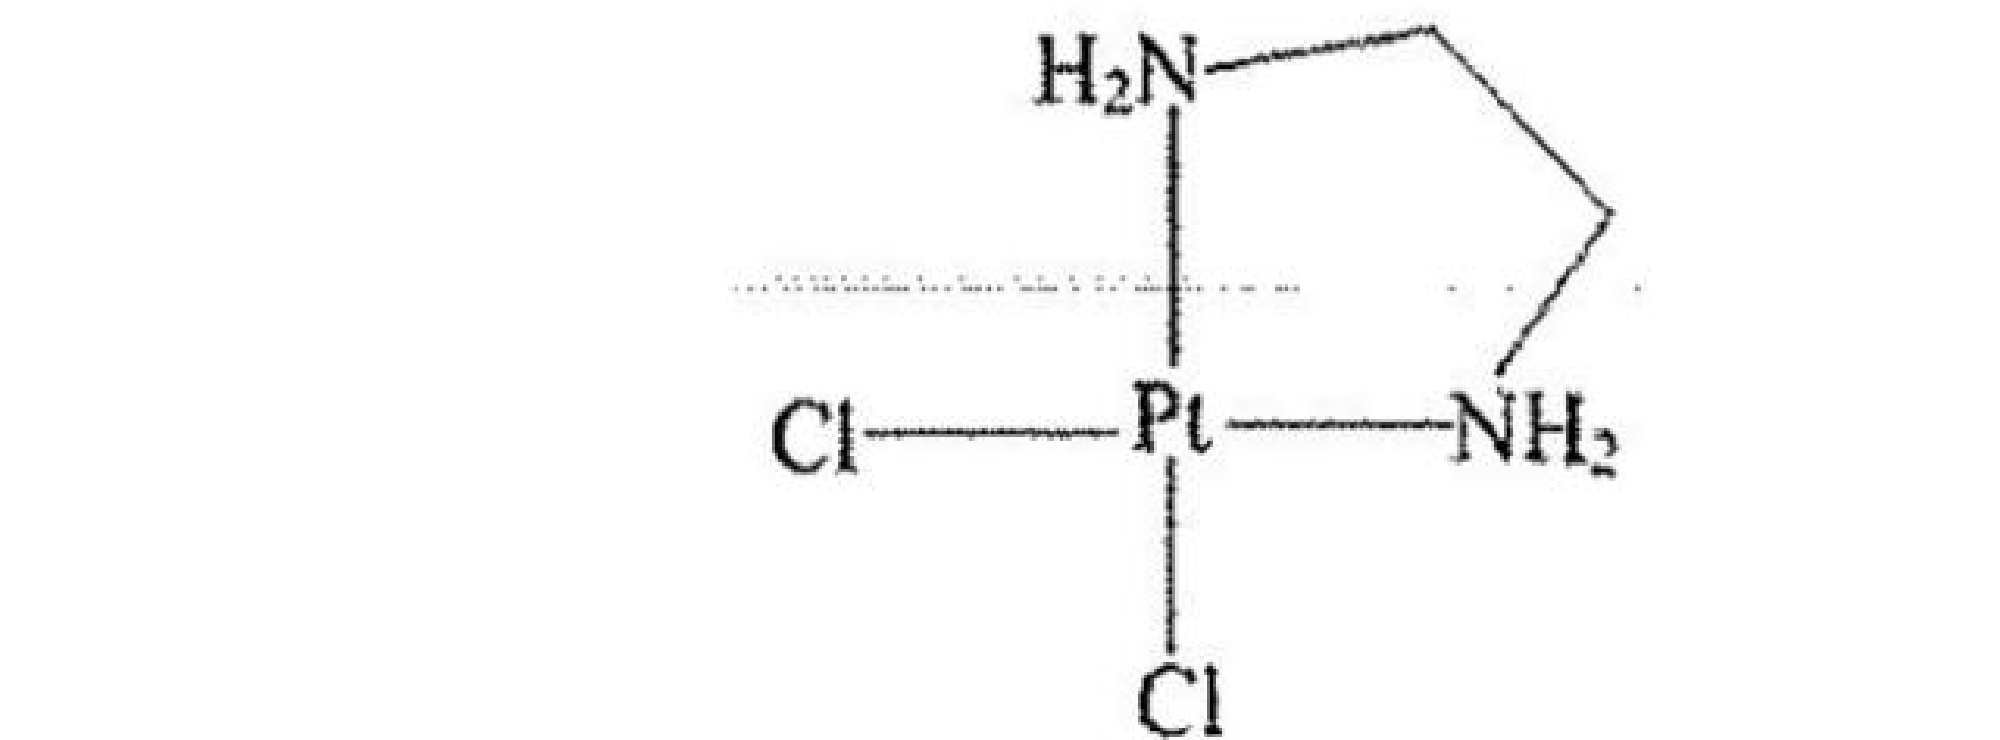
\includegraphics[width=\linewidth]{images_crop_de23/p1_cau14_cis_pt_en.png}
\end{minipage}
\end{ex}

\begin{ex}
EDTA là một phối tử sáu càng có thể tạo phức bát diện bền với hầu hết các cation kim loại theo tỉ lệ mol phối tử : cation là $1 : 1$. Số nguyên tử nitrogen có trong phân tử phối tử EDTA tham gia tạo liên kết phối trí với ion kim loại là
\choice
{2.}
{4.}
{6.}
{8.}
\loigiai{}
\end{ex}

\begin{ex}
Cho sơ đồ chuyển hoá sau:
\par\vspace{1pt}\centerline{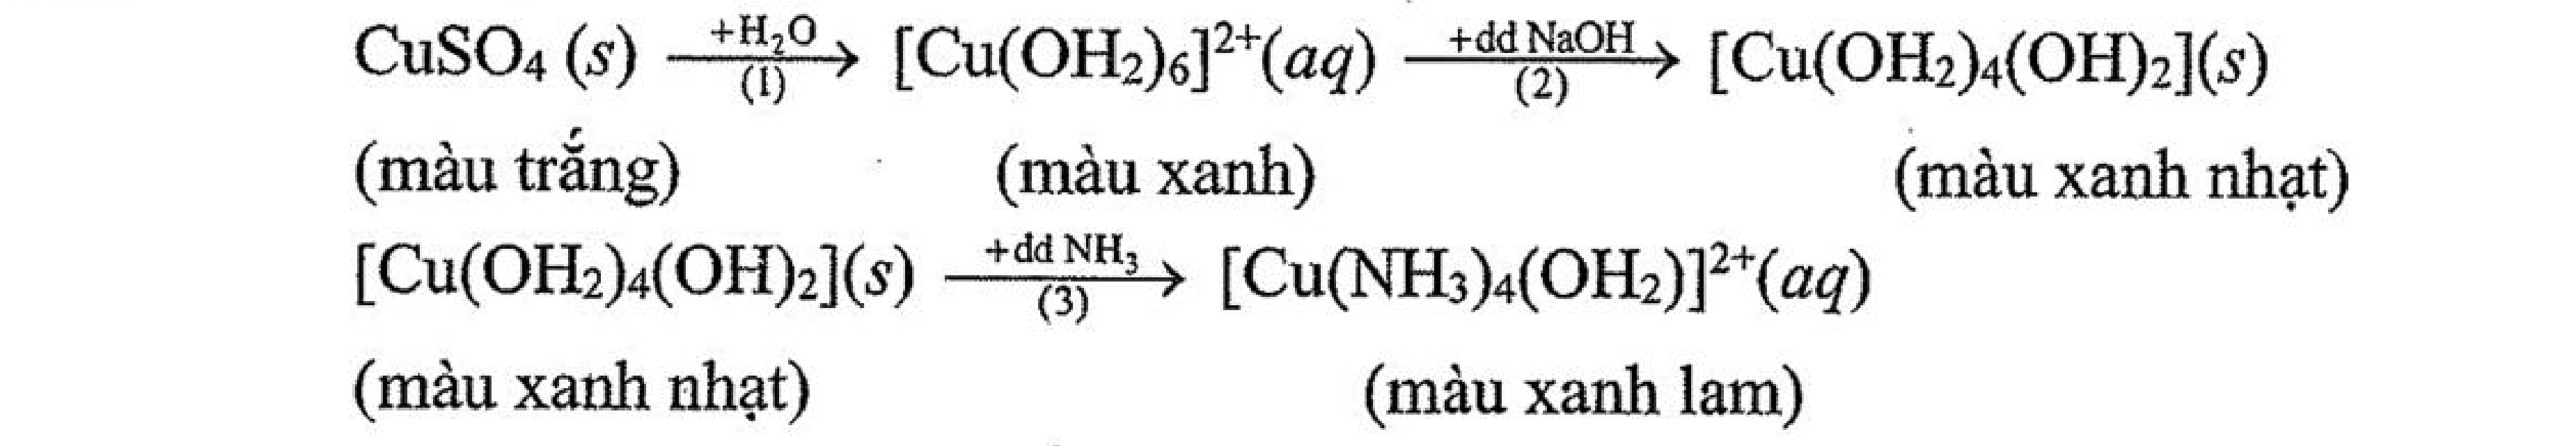
\includegraphics[width=0.55\textwidth]{images_crop_de23/p1_cau16_so_do.png}}\vspace{1pt}
Những phản ứng có sự tạo thành phức chất tan là
\choice
{(1) và (2).}
{(1) và (3).}
{(2) và (3).}
{Cả (1), (2) và (3).}
\loigiai{}
\end{ex}

\begin{ex}
Cho sơ đồ chuyển hoá của bạc (Ag) sau:
\par\vspace{1pt}\centerline{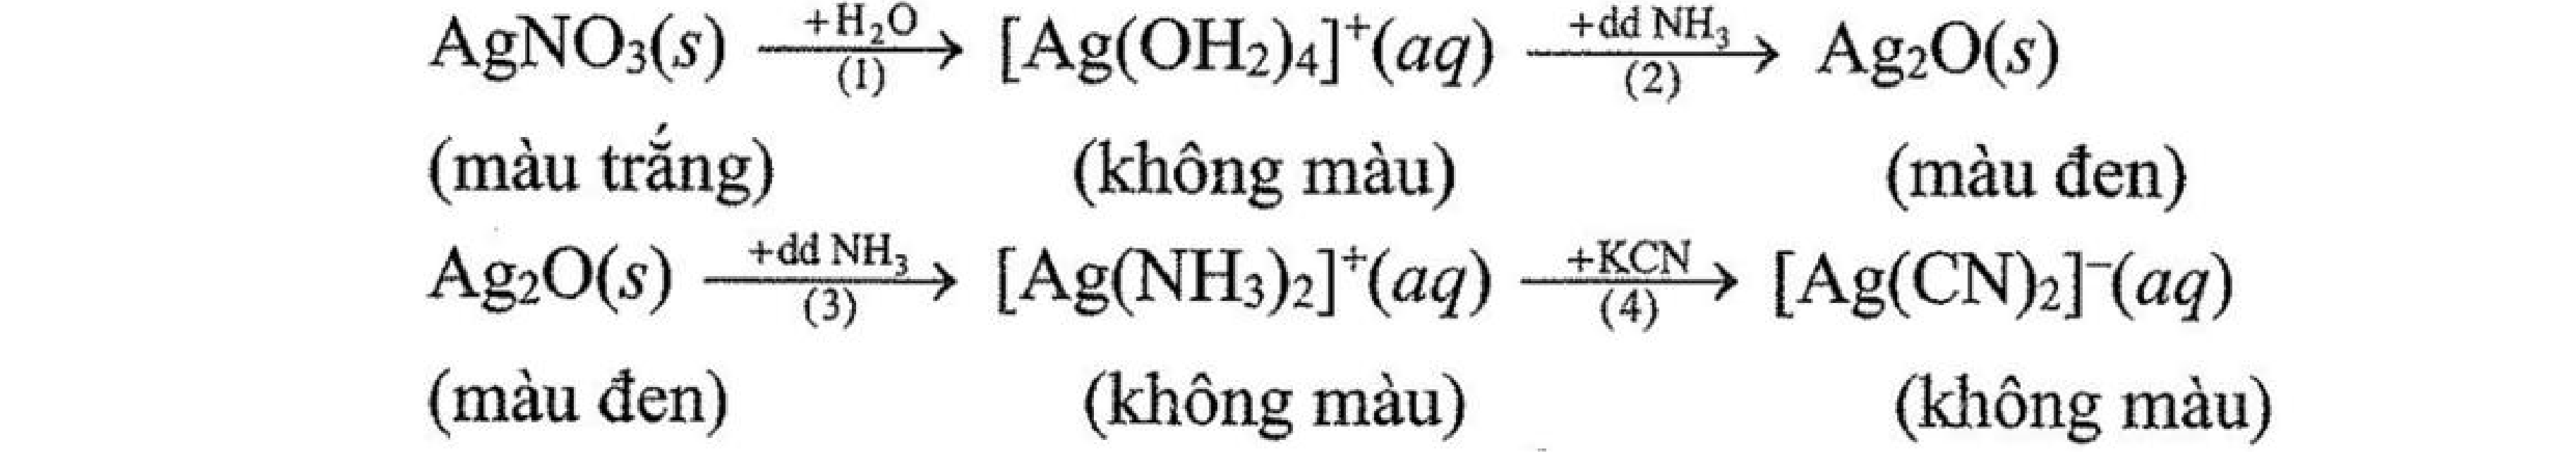
\includegraphics[width=0.55\textwidth]{images_crop_de23/p1_cau17_so_do.png}}\vspace{1pt}
Những phản ứng có sự tạo thành phức chất tan là
\choice
{(1), (2), (3).}
{(1), (3), (4).}
{(2), (3), (4).}
{(1), (2), (4).}
\loigiai{}
\end{ex}

\begin{ex}
Cho cấu hình electron nguyên tử của các nguyên tố: (X): $\text{[Ar]}3d^2 4s^2$; (Y): $\text{[Ar]}4s^1$; (Z): $\text{[Ar]}3d^{10} 4s^2$; (T): $\text{[Ar]}3d^{10} 4s^2 4p^3$. Trong các nhận định sau:\\
(a) Nguyên tố (X) không phải là kim loại chuyển tiếp. \quad (b) Nguyên tố (Y) là kim loại chuyển tiếp.\\
(c) Nguyên tố (T) là kim loại chuyển tiếp. \quad (d) Nguyên tố (Z) không phải là kim loại chuyển tiếp (theo định nghĩa IUPAC).\\
Số nhận định đúng là
\choice
{2.}
{1.}
{3.}
{4.}
\loigiai{}
\end{ex}

\newpage

\noindent
\textbf{PHẦN II (4,0 điểm -- 4 câu): Câu trắc nghiệm đúng sai.}\\
\textit{Thí sinh trả lời từ câu 1 đến câu 4. Trong mỗi ý a), b), c), d) ở mỗi câu, thí sinh chọn đúng hoặc sai.}

\setcounter{ex}{0}

\begin{ex}
[CĐ – SBT] Cho các thông tin về thế điện cực chuẩn của các cặp oxi hoá – khử sau:
\begin{center}
\renewcommand{\arraystretch}{1.1}
\begin{tabular}{|l|c|}
\hline
\textbf{Cặp oxi hoá -- khử} & \textbf{Thế điện cực chuẩn (V)} \\
\hline
$\ce{Fe^3+/Fe^2+}$ & $+0,77$ \\
\hline
$\ce{Cr2O7^2- + 14H+ / 2Cr^3+ + 7H2O}$ & $+1,33$ \\
\hline
$\ce{MnO4- + 8H+ / Mn^2+ + 4H2O}$ & $+1,51$ \\
\hline
\end{tabular}
\end{center}
Biết $\ce{Cr2O7^2-(aq)}$ có màu da cam và $\ce{Cr^3+(aq)}$ có màu xanh lá cây.\\
Xét tính đúng/sai của các phát biểu sau:
\choiceTF
{Trong môi trường acid, anion $\ce{Cr2O7^2-}$ (từ $\ce{K2Cr2O7}$) có tính oxi hoá mạnh hơn anion $\ce{MnO4-}$ (từ $\ce{KMnO4}$).}
{Chuẩn độ được $\ce{Fe^2+}$ trong dung dịch gồm $\ce{Fe^2+}$, $\ce{SO4^2-}$ và $\ce{H+}$ bằng dung dịch chất chuẩn $\ce{KMnO4}$.}
{Không chuẩn độ được $\ce{Fe^2+}$ trong dung dịch gồm $\ce{Fe^2+}$, $\ce{SO4^2-}$ và $\ce{H+}$ bằng dung dịch chất chuẩn $\ce{K2Cr2O7}$.}
{Có diễn ra phản ứng oxi hoá – khử tự diễn biến theo phương trình:\\ $6\ce{Fe^3+}(aq) + 2\ce{Cr^3+}(aq) + 7\ce{H2O}(l) \rightarrow 6\ce{Fe^2+}(aq) + \ce{Cr2O7^2-}(aq) + 14\ce{H+}(aq)$.}
\loigiai{}
\end{ex}

\begin{ex}
[CTST - SBT] Khi tìm hiểu về hợp chất phức chlorophyll (chất diệp lục), xét tính đúng/sai của các phát biểu sau:
\choiceTF
{Chlorophyll chỉ được tìm thấy trong tế bào thực vật.}
{Chlorophyll đóng vai trò hấp thụ năng lượng ánh sáng và xúc tác cho quá trình quang hợp.}
{Trong chất diệp lục chỉ chứa duy nhất một loại chlorophyll.}
{Chlorophyll là thành phần sắc tố quan trọng nhất trong lục lạp của lá cây.}
\loigiai{}
\end{ex}

\begin{ex}
[KNTT - SBT] Nhỏ muối thiocyanate ($\ce{SCN-}$) vào dung dịch muối $\ce{Fe^3+}$ loãng, dung dịch từ màu vàng nhạt chuyển sang màu đỏ máu do một phối tử nước trong phức chất aqua bát diện của $\ce{Fe^3+}$ bị thay thế bởi một phối tử $\ce{SCN-}$:
\choiceTF
{Phức chất aqua của sắt(III) có công thức hoá học là $\ce{[Fe(H2O)6]^3+}$.}
{Phức chất có màu đỏ máu là phức chất của $\ce{Fe^3+}$ chứa 1 phối tử $\ce{SCN-}$ và 6 phối tử nước.}
{Phức chất màu đỏ máu có công thức hoá học là $\ce{[Fe(H2O)5(SCN)]^2+}$.}
{Phức chất màu đỏ máu có điện tích là +3.}
\loigiai{}
\end{ex}

\begin{ex}
Hemoglobin (Hb) là một metalloprotein chiếm khoảng 35\% trọng lượng của hồng cầu, có nhiệm vụ vận chuyển oxygen từ phổi đến các mô. Cấu trúc gồm 4 tiểu đơn vị, mỗi tiểu đơn vị chứa một nhân heme (chiếm 5\% khối lượng Hb) và một chuỗi polypeptide globin. Mỗi nhân heme chứa một ion $\ce{Fe^2+}$ ở trung tâm vòng porphyrin và chỉ liên kết tối đa với 1 phân tử $\ce{O2}$. Đánh giá tính đúng/sai của các phát biểu sau:
\choiceTF
{Dạng hình học của phức chất Fe(II) trong nhân heme khi liên kết với oxygen là bát diện.}
{Mỗi phân tử hemoglobin có thể kết hợp tối đa với bốn phân tử oxygen.}
{Trong các nhân heme, nguyên tử trung tâm $\ce{Fe^2+}$ liên kết với phối tử qua các nguyên tử nitrogen.}
{Trong phân tử hemoglobin, nguyên tố iron (Fe) chiếm 5\% theo khối lượng.}
\loigiai{}
\end{ex}

\newpage

\noindent
\textbf{PHẦN III (1,5 điểm -- 6 câu): Câu trắc nghiệm yêu cầu trả lời ngắn.}\\
\textit{Thí sinh trả lời từ câu 1 đến câu 6.}

\setcounter{ex}{0}

\begin{ex}
Số phối tử không mang điện tích trong phức chất $\ce{[Co(NH3)5Cl]Cl2}$ là bao nhiêu?
\loigiai{}
\end{ex}
\noindent\textit{Trả lời:} \dotfill
\vspace{0.2cm}

\begin{ex}
Số nguyên tử kim loại ở cầu ngoại trong một phân tử phức chất $\ce{Na2[Pt(CN)4]}$ là bao nhiêu?
\loigiai{}
\end{ex}
\noindent\textit{Trả lời:} \dotfill
\vspace{0.2cm}

\begin{ex}
Trong dung dịch nước, ion $\ce{Co^2+}$ tạo thành phức chất aqua có dạng hình học bát diện $\ce{[Co(H2O)6]^2+}$. Số phối tử liên kết với nguyên tử trung tâm trong ion phức này là bao nhiêu?
\loigiai{}
\end{ex}
\noindent\textit{Trả lời:} \dotfill
\vspace{0.2cm}

\begin{ex}
Cho các phức chất và ion phức sau: $\ce{[Co(NH3)6]^3+}$, $\ce{[Cr(H2O)6]^3+}$, $\ce{[Ni(CO)4]}$, $\ce{[BF4]-}$, $\ce{[Fe(CN)6]^4-}$, $\ce{[Ag(NH3)2]+}$. Có bao nhiêu phức anion (phức chất mang điện tích âm) trong số các chất trên?
\loigiai{}
\end{ex}
\noindent\textit{Trả lời:} \dotfill
\vspace{0.2cm}

\begin{ex}
Cho 16,0 gam bột CuO tan hết trong dung dịch $\ce{H2SO4}$ 20\% vừa đủ, sau đó làm nguội dung dịch thu được đến 10$^\circ$C thấy tách ra $m$ gam tinh thể $\ce{CuSO4.5H2O}$. Biết độ tan của $\ce{CuSO4}$ ở 10$^\circ$C là 17,4 gam trong 100 gam nước. Giá trị của $m$ là bao nhiêu? \textit{(Làm tròn kết quả đến hàng phần mười)}.
\loigiai{}
\end{ex}
\noindent\textit{Trả lời:} \dotfill
\vspace{0.2cm}

\begin{ex}
Đem 9,80 gam muối Mohr $\ce{FeSO4.(NH4)2SO4.6H2O}$ hoà tan trong nước cất rồi định mức thành 250 mL dung dịch trong bình định mức với sự có mặt của $\ce{H2SO4}$ loãng. Tiến hành chuẩn độ 25,0 mL dung dịch này bằng dung dịch $\ce{KMnO4}$ chưa rõ nồng độ, thể tích dung dịch $\ce{KMnO4}$ tiêu tốn trung bình qua 3 lần chuẩn độ là 24,65 mL. Nồng độ mol/L của dung dịch $\ce{KMnO4}$ là bao nhiêu? \textit{(Làm tròn đến hai chữ số thập phân)}.
\loigiai{}
\end{ex}
\noindent\textit{Trả lời:} \dotfill
\vspace{0.2cm}

\Closesolutionfile{ans}


\end{document}
